%!TEX root = ../AutoML-fuer-Segmentierung.tex
\chapter{nnUNet}
\label{ch:nnunet}


\section{Funktionsweise / Theorie}


\label{tab:multicol}

Das nnU-Net ist ein Framework, welches sich mit der Segmentierung von medizinischen 3D-Aufnahmen mit Hilfe von automatisiertem maschinellem Lernen beschäftigt. Es wurde im Rahmen des Medical Segmentation Decathlon Wettbewerb entwickelt und gewann diesen sowie im Anschluss auch viele weitere Segmentierungs-Wettbewerbe. \\
Das nnU-Net verwendet eine klassische und nicht neue U-Net Architektur (not new U-Net). Es konzentriert sich kaum auf  Architekturdesign und -suche, sondern vorrangig auf die Suche von guten Hyperparametern. Es wird eine gleiche oder sehr ähnliche U-Net Struktur immer durch eine individuell auf die individuellen Daten angepasste Trainingspipeline zur Optimierung geschickt (siehe Abbildung \ref{pic:nnUnet_Basisschema}). Das Training der Parameter des Netzes ist also individuell zugeschnitten, während die Architektur sich bei unterschiedlichen Daten nicht oder kaum unterscheidet. Es wird sich also vorrangig auf das Training des Netzes und die Suche individueller Hyperparameter für die Trainingspipeline konzentriert und nicht auf die Suche nach der Architektur. 

\begin{figure}[H]
	
	\centering
	
\includegraphics[scale=0.3]{Pictures/nnUnet/Bild01.png}
	\caption{}
	\label{pic:nnUnet_Basisschema}
\end{figure}



Das nnU-Net verwendet 3 Standardarchitekturen, welche 2D U-Net, 3D full resolution U-Net und 3D U-Net Cascade sind. Vor dem Training kann man einstellen, wie viele und welche Architekturen man trainieren möchte. Per default trainiert nnU-Net alle und wählt am Ende die beste oder die beste Kombination aus maximal zwei Architekturen aus. 2D U-Net eignet sich besonders für 2D-Daten und läuft gut auf anisotropen Daten. Es arbeitet auf den Bildern in Originalauflösung. 3D full resolution U-Net eignet sich für kleine 3D-Daten und arbeitet auch auf den Bildern in Originalauflösung. Bei größeren Bildern werden jedoch die Patches sehr klein, was zum immer größer werdenden Verlust von Kontextdaten führt. Daher gibt es das 3D U-Net Cascade für große 3D-Daten. Es besteht aus 2 hintereinander gereihten U-Nets. Das erste U-Net arbeitet auf den Bildernals ganzes, also ohne Aufteilung in Patches, in geringerer Auflösung. Diese grobe Vorsegmentierung wird zusammen mit dem Bild in Originalgröße an das zweite U-Net weitergegeben. Dieses arbeitet dann wieder auf der vollen Bildauflösung und mit Patches und erstellt eine endgültige und verfeinerte Segmentierung. Durch diesen Übergabeschritt zwischen den beiden U-Nets bleiben die Kontextdaten erhalten (siehe Abbildung \ref{pic:nnUnet_Cascade}).

\begin{figure}[H]
	
	\centering
	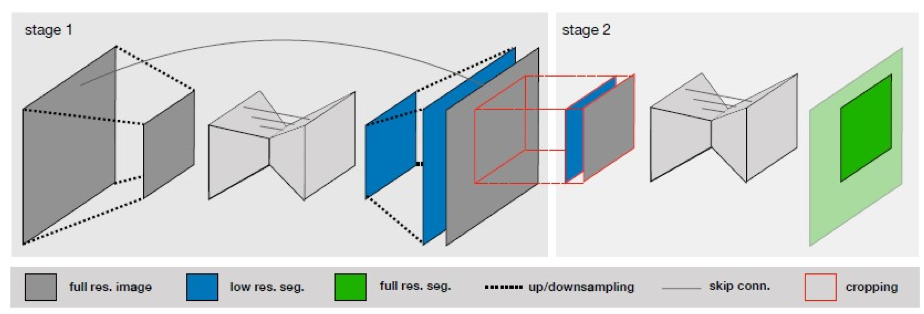
\includegraphics[scale=0.8]{Pictures/nnUnet/Bild02.png}
	\caption{nnU-Net Cascade \cite{nnunetPaper} }
	\label{pic:nnUnet_Cascade}
\end{figure}


Um die Konzentration auf die Anpassung der Hyperparameter der Trainingspipeline an den individuellen Datensatz zu erreichen, wird zunächst ein Datafingerprint aus den Eigenschaften der Trainingsdaten erstellt (siehe Abbildung \ref{pic:nnUnet_Datafingerprint}). Die hierbei genutzten Eigenschaften sind unter anderem die Imgasize, das Pixelvolumen oder die Farbkanäle, die spacing Anisotropie sowie die Anzahl der Klassen und deren Häufigkeitsverteilung. 

\begin{figure}[H]
	
	\centering
	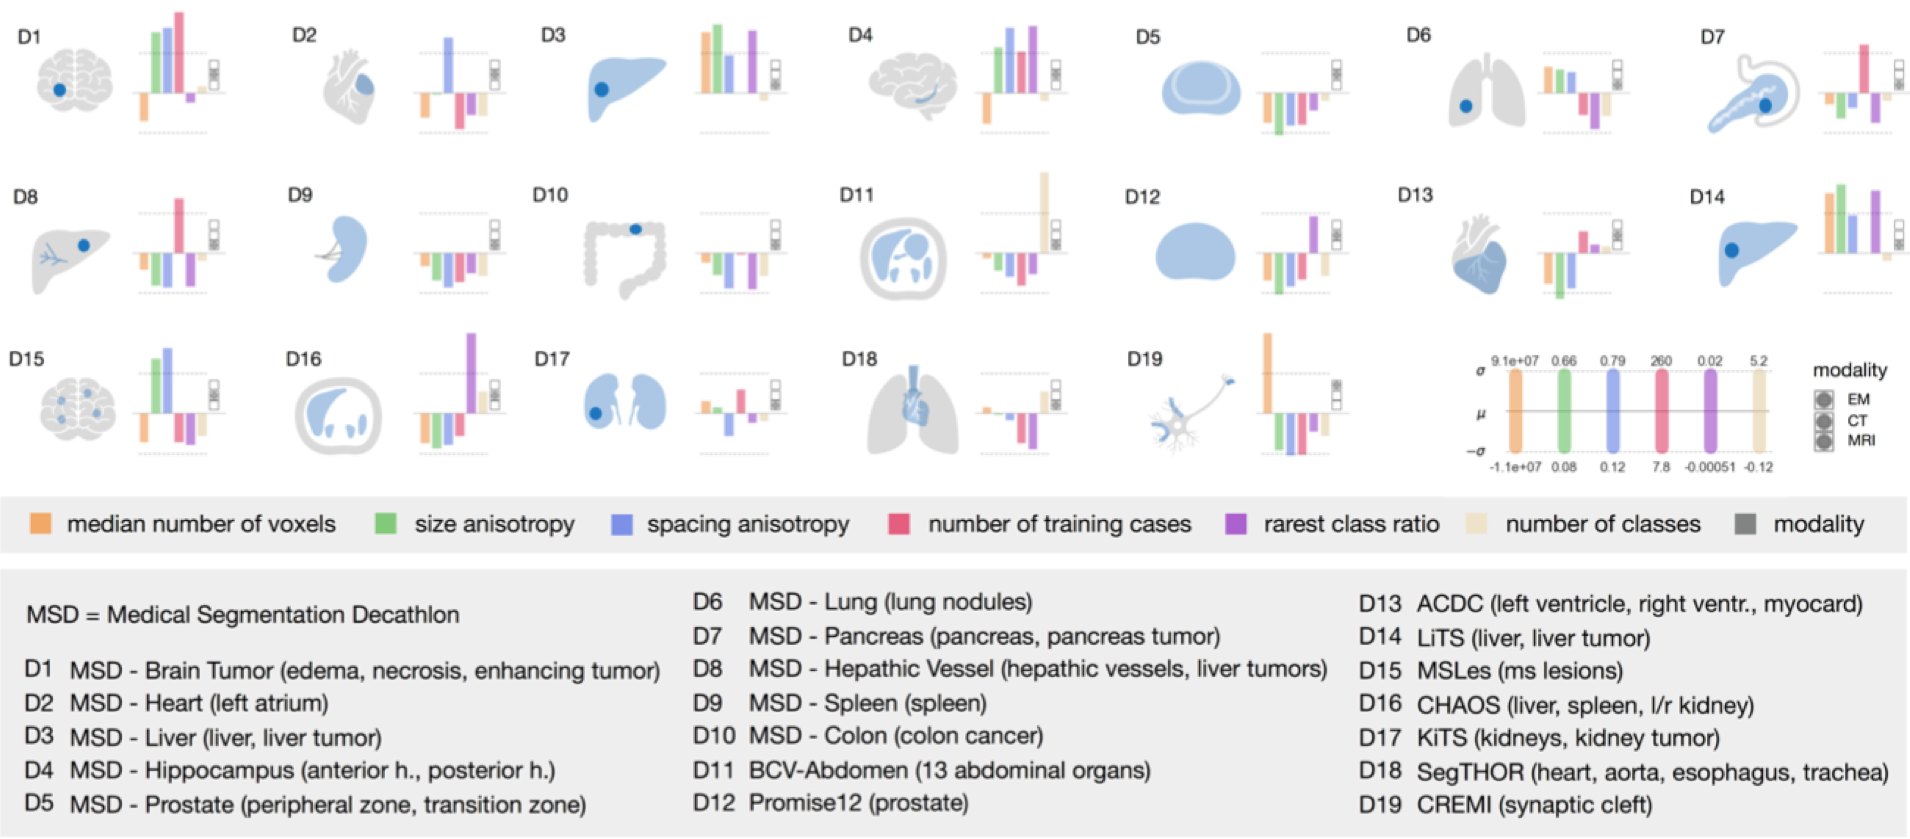
\includegraphics[scale=0.45]{Pictures/nnUnet/Bild03.png}
	\caption{Datafingerprint \cite{nnunetPaperB}}
	\label{pic:nnUnet_Datafingerprint}
\end{figure}


Aus dem Datafingerprint werden, mit Hilfe von heuristischen Regeln, die Inferred Parametern berechnet. Die Inferred Parameter umfassen die Patch Size, die Batch size, wichtige Parameter zur dynamischen Anpassung der Netzwerktopologie, wie zum Beispiel die Anzahl der Max. Poolings und Downsamplings, sowie Parameter zur Bild Vorverarbeitung. \\
Die Bestimmung der Patch size erfolgt zunächst initial über den Median der Bildgröße nach dem Resampling. Anschließend wird mit dieser Patch Size die Architektur konfiguriert und geschaut ob ausreichend GPU-Memory zur Verfügung steht. Steht nicht ausreichend GPU-Memory zur Verfügung, so wird die Patch Size reduziert und die Architektur darauf aufbauend neu konfiguriert. Dies wird so oft wiederholt, bis ausreichend GPU-Memory verfügbar ist. Anschließend wird die Batch Size angepasst und das Netzwerk abschließend konfiguriert (Siehe Abbildung \ref{pic:nnUnet_PatchSize}). Dabei muss beachtet werden, dass die Patch Size immer durch $2^i$ teilbar sein muss (mit i = Anzahl an Downsampling Operationen) da sich die Patch Size pro Downsampling Operation halbiert. Ist das nicht gegeben, so wird die Patch-Size entsprechend vergrößert oder verkleinert bis sie in allen Dimensionen durch $2^i$ teilbar ist.
 
 \begin{figure}[H]
 	
 	\centering
 	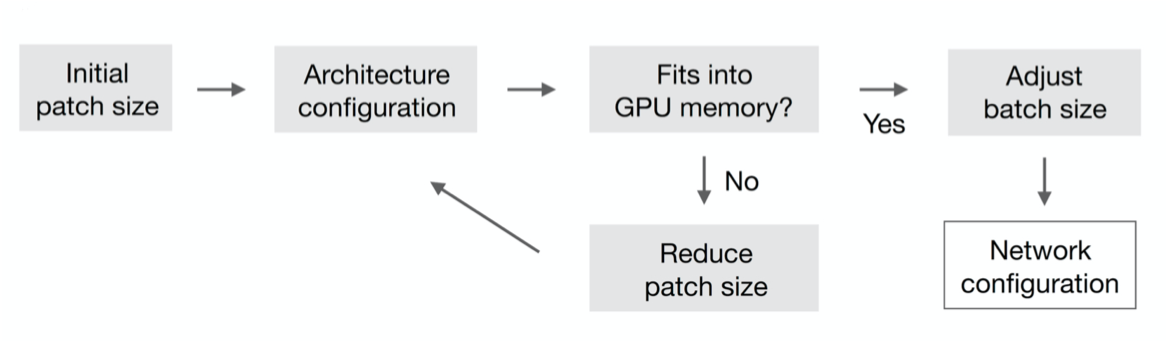
\includegraphics[scale=0.6]{Pictures/nnUnet/Bild04.png}
 	\caption{Patch Size Ermittlung \cite{nnunetPaperB} }
 	\label{pic:nnUnet_PatchSize}
 \end{figure}
 

Im Anschluss an die Inferred Parameter wird der Pipelinefingerprint erstellt, welcher sich aus den Inferred Parametern, den Blueprint Parametern und den empirischen Parametern zusammensetzt. Während die bereits beschriebenen Inferred Parameter für die entscheidende Anpassung an einen neuen Datensatz sorgen, sind die Blueprint Parameter unabhängig von dem Datensatz. Sie enthalten die drei möglichen Architekturen, sowie Hyperparameter mit festen default Werten, wie Verlustfunktion, Training Schedule, Data Augmentation, Normalisierung, stochastic Gradient oder  Aktivierungsfunktion (siehe Abbildung \ref{pic:nnUnet_Pipelinefingerprint}). Die Verlustfunktion wird als die Summe von Dice-Verlustfunktion und Cross-Entropy-Verlustfunktion gewählt. Dies wird gemacht, da medizinische Bilddaten oft Probleme mit einer großen Disbalance im Vorkommen der einzelnen Klassen haben und darum im Training seltener vorkommende Klassen unterepräsentiert sind und gleichzeitig durch die Lösung dieses Problems die Verteilung der Klassen verzerrt wird. An der Zusammensetzung dieser beiden Verlustfunktionen könnte man also auch arbeiten, wenn man das Framework auf andere Arten von Datensätzen anpassen wollte. Das Training läuft über 1000 Epochen mit jeweils 250 Trainingsiterationen. 

\begin{figure}[H]
	
	\centering
	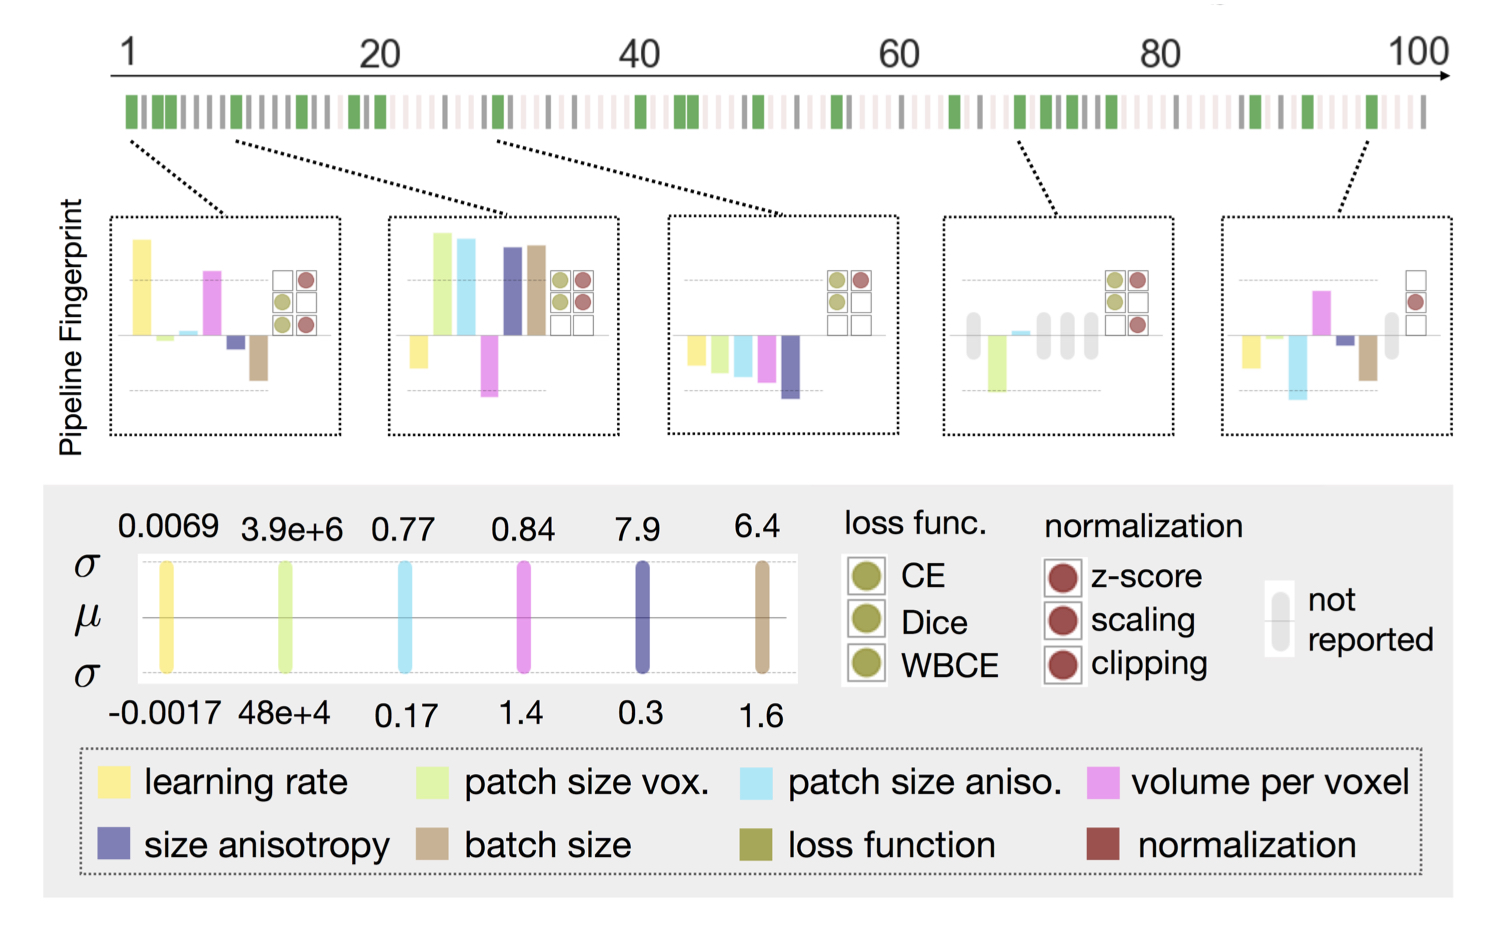
\includegraphics[scale=0.5]{Pictures/nnUnet/Bild05.png}
	\caption{Pipelinefingerprint \cite{nnunetPaperB} }
	\label{pic:nnUnet_Pipelinefingerprint}
\end{figure}

Da die empirischen Parameter nicht direkt aus dem Datensatz erschlossen werden können, werden sich nach dem Training empirisch bestimmt. Sie werden zur Nachbearbeitung und bei der Auswahl der besten Netzstruktur genutzt. 


\section{Unsere Arbeit / Praxis}




\section{Ergebnisse}


\section{Fazit}

